\subsection{Mathematical Formulation}

The Regression Monte Carlo (RMC) approach for pricing convertible bonds is based on the Longstaff-Schwartz algorithm. This method uses simulation paths and regression to estimate continuation values, allowing for efficient pricing of early exercise features.

At each potential conversion date, the bondholder must decide whether to convert by comparing:
\begin{itemize}
    \item The immediate conversion value: $\ell S(t)$
    \item The continuation value: $\mathbb{E}[V(t+\Delta t, S(t+\Delta t)) | S(t)]$
\end{itemize}

The algorithm proceeds as follows:

\begin{enumerate}
    \item Generate $N$ paths of the stock price process under the risk-neutral measure:
    \begin{equation}
        dS(t) = rS(t)dt + \sigma S(t)dW(t)
    \end{equation}
    
    \item Initialize terminal cash flows at maturity $T$:
    \begin{equation}
        V_i(T) = \max(N, \ell S_i(T)) \quad \text{for } i = 1, 2, \ldots, N
    \end{equation}
    
    \item Working backward in time, at each potential conversion date $t_j$:
        \begin{itemize}
            \item Identify paths where conversion is in-the-money: $\ell S_i(t_j) > 0$
            \item For these paths, estimate the continuation value using regression:
            \begin{equation}
                \hat{C}_i(t_j) = \sum_{k=0}^{M} \beta_k \phi_k(S_i(t_j))
            \end{equation}
            where $\phi_k$ are basis functions (polynomials) and $\beta_k$ are regression coefficients
            \item Compare the estimated continuation value with the immediate conversion value:
            \begin{equation}
                V_i(t_j) = \max(\hat{C}_i(t_j), \ell S_i(t_j))
            \end{equation}
            \item Add coupon payments if $t_j$ is a coupon date:
            \begin{equation}
                V_i(t_j) = V_i(t_j) + K N \Delta t
            \end{equation}
            \item Discount cash flows to the previous time step:
            \begin{equation}
                V_i(t_{j-1}) = e^{-r(t_j-t_{j-1})}V_i(t_j)
            \end{equation}
        \end{itemize}
        
    \item The convertible bond price at $t=0$ is the average of discounted cash flows:
    \begin{equation}
        V(0) = \frac{1}{N}\sum_{i=1}^{N}V_i(0)
    \end{equation}
\end{enumerate}

\subsection{Implementation Results}

Using the Regression Monte Carlo approach with the same parameters, but simulating daily:
\begin{itemize}
    \item Initial stock price: $S_0 = 200$
    \item Face value: $N = 1000$
    \item Conversion ratio: $\ell = 3$
    \item Annual coupon rate: $K_{\text{coupon}} = 0.016$
    \item Risk-free rate: $r = 0.03$
    \item Volatility: $\sigma = 0.3$
    \item Maturity: $T = 5$ years
    \item Number of simulation paths: $n_{\text{paths}} = 10,000$
    \item Number of time steps: $n_{\text{steps}} = 252 \times 5$ (daily steps)
    \item Polynomial regression degree: 3
\end{itemize}

The computed price of the convertible bond at $t = 0$ is:
\begin{equation}
    V(0, S_0) = 1064.9177
\end{equation}

This represents a conversion premium of 6.49\% over the face value, reflecting the embedded option value of the conversion feature.

\begin{figure}[H]
    \centering
    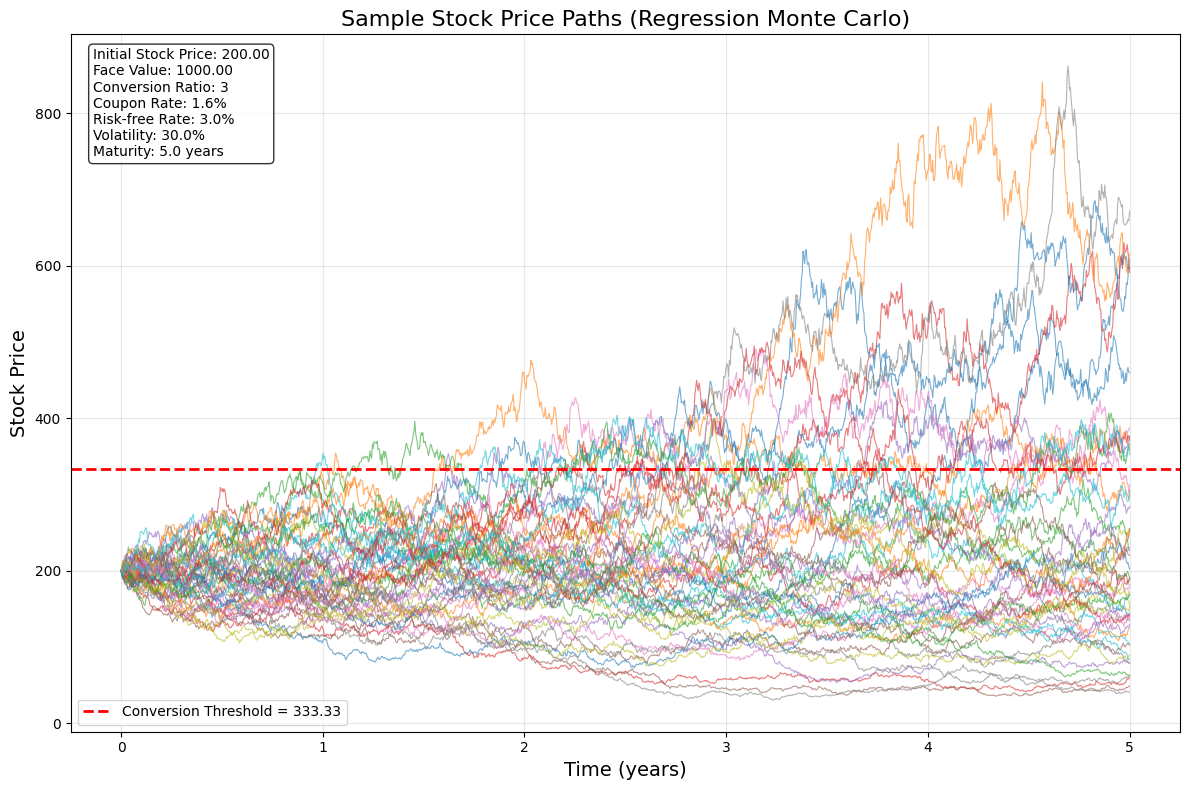
\includegraphics[width=0.75\textwidth]{img/02_sample_paths.png}
    \caption{Sample stock price paths under the risk-neutral measure. The horizontal red line represents the conversion threshold $N/\ell = 333.33$.}
    \label{fig:sample_paths}
\end{figure}

Figure \ref{fig:sample_paths} shows sample stock price paths generated under the risk-neutral measure. The horizontal red line represents the conversion threshold $N/\ell = 333.33$, which is the stock price at which the conversion value equals the face value of the bond.

\begin{figure}[H]
    \centering
    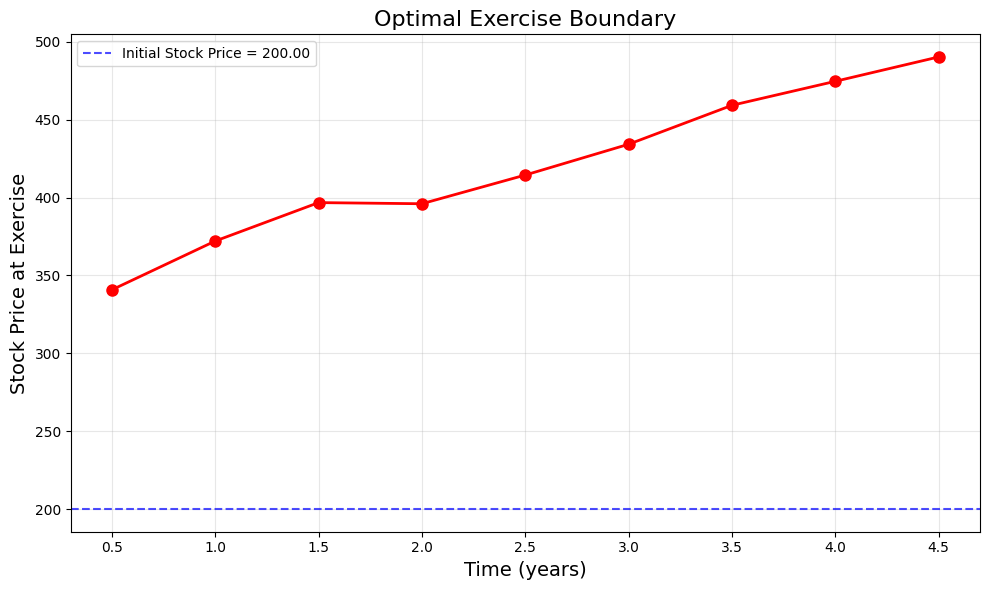
\includegraphics[width=0.75\textwidth]{13_ConvertibleBonds/img/02_optimal_exercise_bound.png}
    \caption{Optimal exercise boundary showing the stock price threshold above which early conversion is optimal at each conversion date.}
    \label{fig:exercise_boundary}
\end{figure}

\subsection{Sensitivity Analysis}

The convertible bond price is sensitive to various market parameters. Figure \ref{fig:sensitivity_analysis} illustrates how the bond price varies with volatility, stock price, and interest rate.

\begin{figure}[h!]
    \centering
    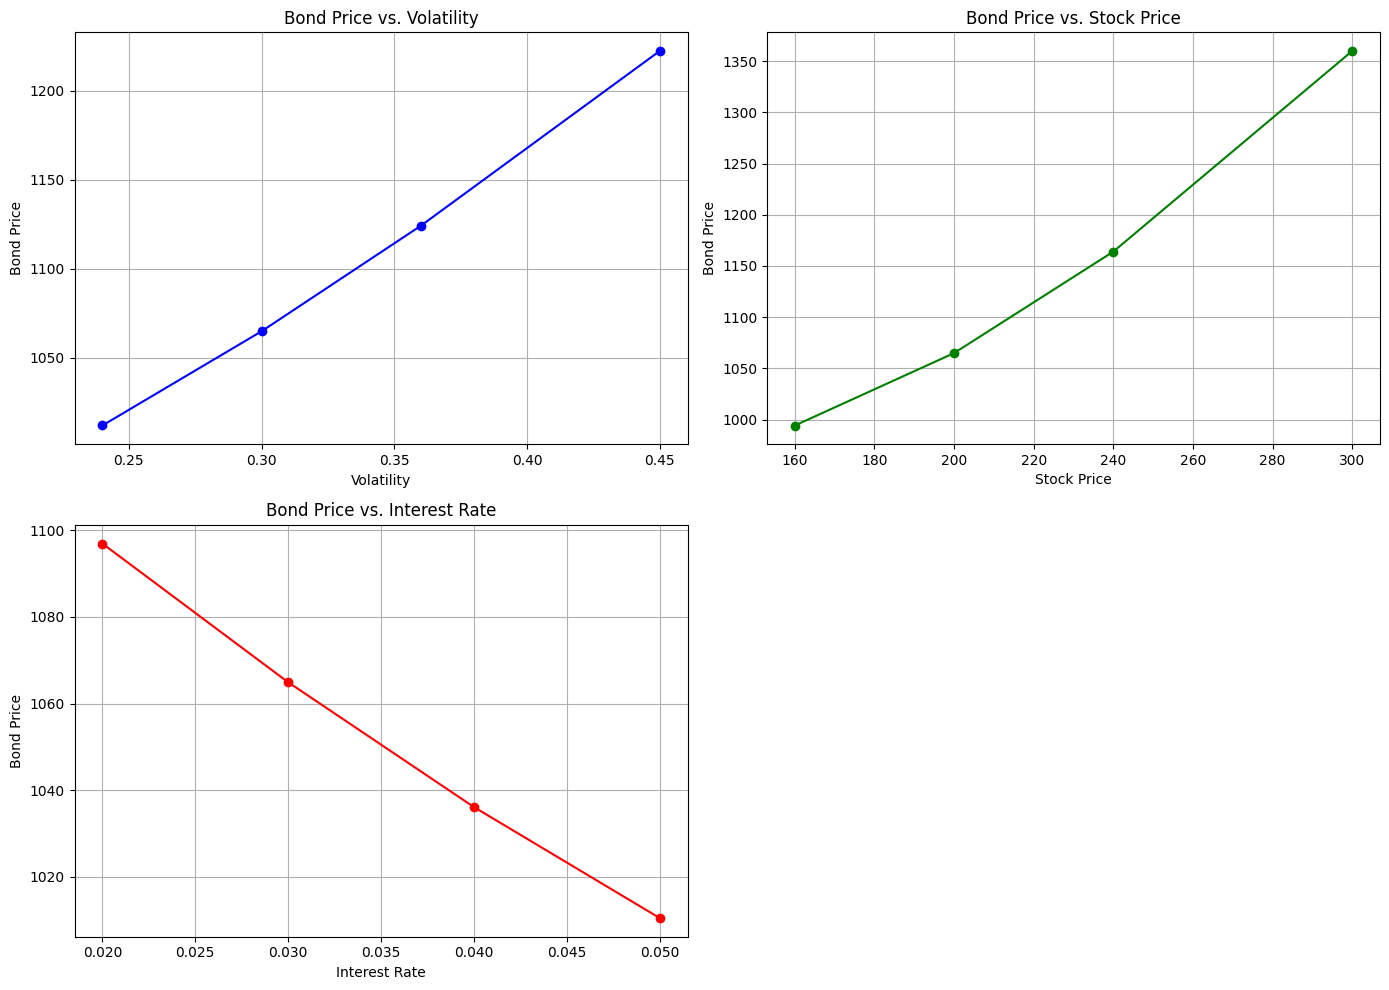
\includegraphics[width=0.8\textwidth]{13_ConvertibleBonds/img/02_sensitivity_analysis.png}
    \caption{Sensitivity of convertible bond price to volatility, stock price, and interest rate.}
    \label{fig:sensitivity_analysis}
\end{figure}

\subsubsection{Volatility Sensitivity}

Increasing volatility increases the convertible bond price, as shown in the top-left panel of Figure \ref{fig:sensitivity_analysis}. This occurs because higher volatility increases the probability of the stock price exceeding the conversion threshold, enhancing the value of the conversion option. Specifically:

\begin{itemize}
    \item At $\sigma = 24\%$: Bond price = 1011.99 ($\Delta$ = -52.93)
    \item At $\sigma = 30\%$: Bond price = 1064.92 (base case)
    \item At $\sigma = 36\%$: Bond price = 1124.17 ($\Delta$ = +59.25)
    \item At $\sigma = 45\%$: Bond price = 1222.29 ($\Delta$ = +157.37)
\end{itemize}

The relationship is non-linear, with larger increases in bond price as volatility increases, demonstrating the convex nature of the option component.

\subsubsection{Stock Price Sensitivity}

The convertible bond price is highly sensitive to the underlying stock price, as shown in the top-right panel of Figure \ref{fig:sensitivity_analysis}. Higher stock prices increase the probability of profitable conversion, thereby increasing the bond value:

\begin{itemize}
    \item At $S_0 = 160$: Bond price = 994.18 ($\Delta$ = -70.74)
    \item At $S_0 = 200$: Bond price = 1064.92 (base case)
    \item At $S_0 = 240$: Bond price = 1164.00 ($\Delta$ = +99.08)
    \item At $S_0 = 300$: Bond price = 1359.88 ($\Delta$ = +294.96)
\end{itemize}

When the stock price is low ($S_0 = 160$), the bond trades below par value, indicating that the market expects the bond to be redeemed at face value rather than converted. As the stock price increases, the bond price increases at an accelerating rate, reflecting the increasing probability of conversion.

\subsubsection{Interest Rate Sensitivity}

The convertible bond price decreases as interest rates increase, as shown in the bottom-left panel of Figure \ref{fig:sensitivity_analysis}:

\begin{itemize}
    \item At $r = 2\%$: Bond price = 1096.91 ($\Delta$ = +31.99)
    \item At $r = 3\%$: Bond price = 1064.92 (base case)
    \item At $r = 4\%$: Bond price = 1036.12 ($\Delta$ = -28.80)
    \item At $r = 5\%$: Bond price = 1010.52 ($\Delta$ = -54.40)
\end{itemize}

This negative relationship arises from two competing effects:
\begin{enumerate}
    \item Higher interest rates reduce the present value of future cash flows (coupon payments and principal), decreasing the bond component value.
    \item Higher interest rates increase the expected growth rate of the stock price under the risk-neutral measure, potentially increasing the conversion option value.
\end{enumerate}

In this case, the first effect dominates, resulting in a negative relationship between interest rates and bond price.
